%Bias-variance tradeoff: bias-variance decomposition (derivation and interpretation of the different terms, link with over- and under-fitting), parameters that influence bias and variance, bias and variance estimation

\newpage
\section{Bias-variance tradeoff}
L'erreur qu'un algo veut minimizer est: 
$$E = \textcolor{blue}{VAR_y\{y\}} +  \textcolor{teal}{Bias^2} + \textcolor{red}{VAR_{LS}\{\hat y\}}$$
où
\begin{itemize}
    \item \textcolor{blue}{$VAR_y\{y\}$} = à \textcolor{blue}{\textbf{l'erreur résiduel}} ou encore l'erreur minimal atteignable
    \item \textcolor{blue}{$VAR_y\{y\} = E_y\{(y-E_y\{y\})^2\}$}
    \item $\textcolor{teal}{Bias^2}$ = erreur between Bayes and average model
    \item $\textcolor{teal}{Bias^2 =  (E_y\{y\}- E_{LS}\{\hat{y}\})^2}$
    \item $E_{LS}\{\hat{y}\}$ = average model (over all LS)
    \item $\textcolor{red}{VAR_{LS}\{\hat y\}}$ = estimation of variance, consequence of
    over-fitting
    \item $\textcolor{red}{VAR_{LS}\{\hat y\} = E_{LS}\{(\hat{y}-E_{LS}\{\hat{y}\})^2\}}$
\end{itemize}

\begin{figure}[H]
    \centering
    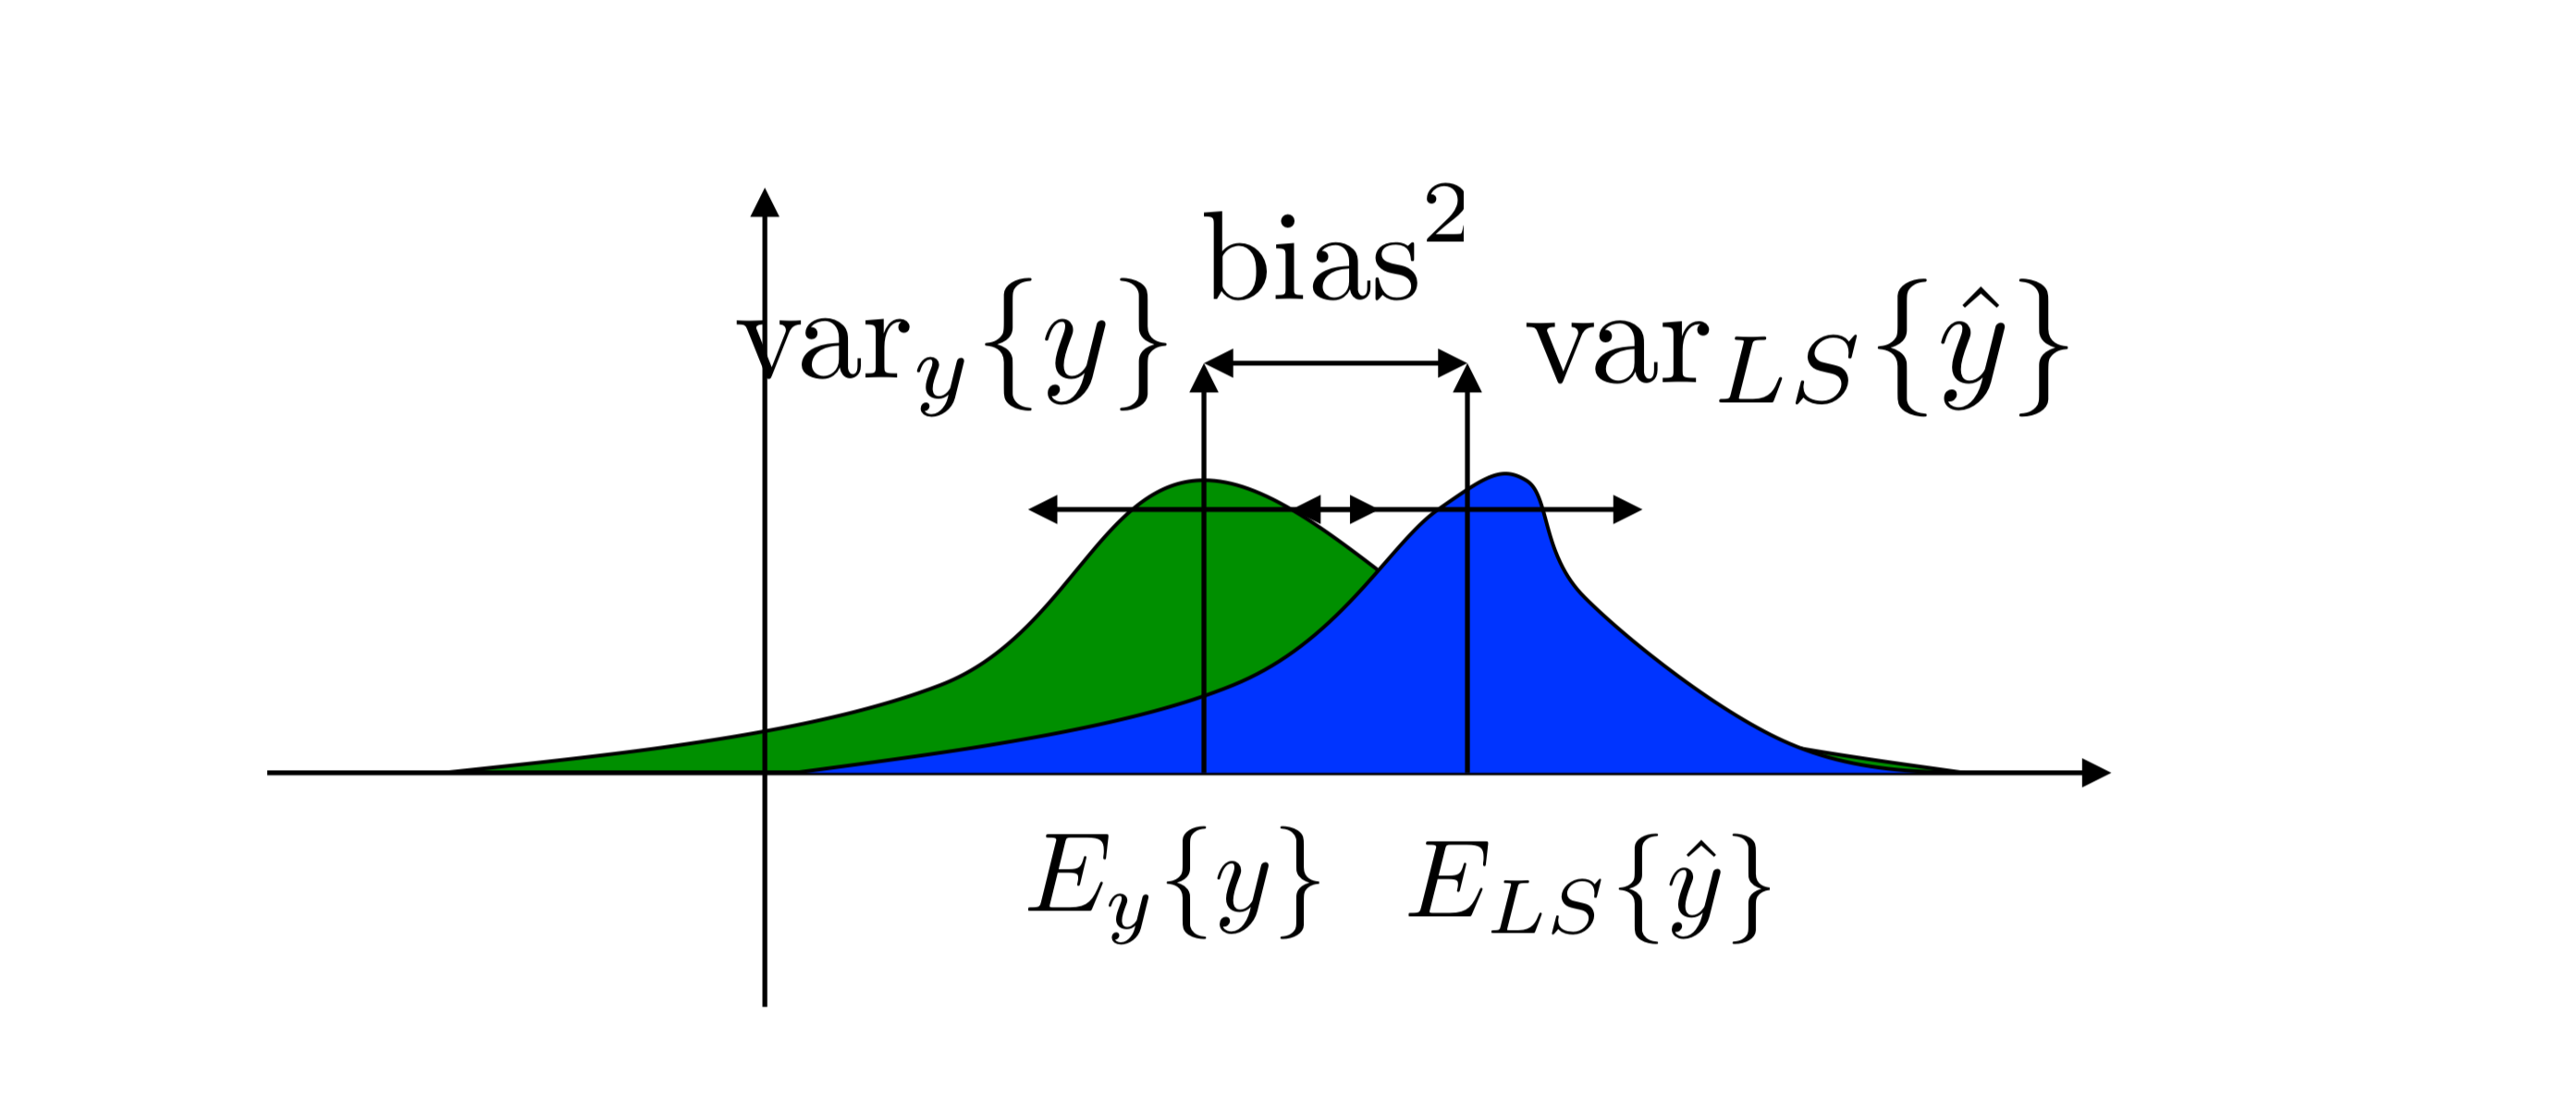
\includegraphics[scale = 0.3]{Question4/bias-variance.png}
    \caption{Caption}
    \label{fig:my_label}
\end{figure}
L'erreur mentionnée précédemment était dans le cas d'absence d'entrées.
Pour plusieurs entrées, l'erreur qu'un bon algorithme d'apprentissage devrait minimiser est:
$$E = E_{LS}\{E_{\overline{x},y}\{(y-\hat{y}(x))^2\}$$
et puisque $ E_{\overline{x},y}\{....\} = E_{\overline{x}}\{E_{y|\overline{x}}\{....\}\}$, il vient: 
$$ E = 
 \textcolor{blue}{E_{\overline{x}}\{VAR_{y|\overline{x}}\{y\}\}}
+ \textcolor{teal}{ E_{\overline{x}}\{Bias^2(\overline{x}\}}
+  \textcolor{red}{ E_{\overline{x}}\{VAR_{LS}\{\hat{y}(\overline{x}\}\} }
$$

\begin{itemize}
    \item  $\textcolor{blue}{VAR_{y|\overline{x}}\{y\}}$ is the \textbf{noise} $\rightarrow$ \textcolor{blue}{How much "y" vary from Bayes Model}.
    \item $\textcolor{teal}{ Bias^2(\overline{x})}$ $\rightarrow$ \textcolor{teal}{Measure error btw Bayes model \& average model}.
    \item $\textcolor{red}{ VAR_{LS}\{\hat{y}(\overline{x}\}}$ $\rightarrow$ \textcolor{red}{ How much "$f(\overline{x})$ "vary from one LS to another}.
\end{itemize}
\subsection{Low variance \& High Biais}
Your model is far from the bayes model (BIg error) the learning algo is giving the same model $\approx$ watever the LS $\rightarrow$ \textbf{Under-fitting}
\subsection{Low Biais \& High variance}
Your model is close to the bayes model for the objects in the LS (low error) but your model is highly dependent of your LS $\rightarrow$ \textbf{Over-fitting}
\subsection{Parameter that influence Biais \& variance}
\begin{itemize}
    \item Complexity of the Model $\nearrow$ $\Rightarrow$ \textcolor{teal}{\textbf{Biais}} $\searrow$ \&  \textcolor{red}{\textbf{variance}} $\nearrow$
    \item Complexity of Bayes model $\nearrow$ $\Rightarrow$ \textcolor{teal}{\textbf{Biais}} $\searrow$ \& no behavior of \textcolor{red}{\textbf{variance}}
    \item \textcolor{blue}{\textbf{Noise}}  $\nearrow$ \Rightarrow \textcolor{red}{\textbf{variance}} $\nearrow$  $\Rightarrow$  \textcolor{teal}{\textbf{Biais}} $\approx$ unafflected
    \item \textbf{LS} $\nearrow$ $\Rightarrow$ $\Biais$ $\approx$ unafflected and $\variance$ $\nearrow$ ($\noise$  has less impact)
\end{itemize}
Learning algo:
\begin{itemize}
    \item $\linreg$ : Hight $\Biais$ \& small $\variance$
    \item $\regtr$: Small $\Biais$ \& Hight $\variance$
    \item \textbf{knn}
    \begin{itemize}
        \item k=1: Moderate $\Biais$ \& hight $\variance$
        \item k=10: Moderate $\Biais$ \& small $\variance$
    \end{itemize}
\end{itemize}